\chapter{Comparison among Different Image Classification Neural Nets}
% Authors: Danfeng Li, Zexi Ye, Wei-Yun Wang 3/12/19.
The age of information explosion is characterized by an overflow of data in all forms. Images, in particular, are among one of the most common types of unstructured data. Nowadays, deep neural networks prove to be an excellent model for making sense of images. One crucial objective of these models is to classify the object that appears in an image. Nevertheless, training a deep neural network is an arduous task. It entails the following:

\begin{enumerate}
    \item \textbf{Computational Power.}
    Training a neural network is a computationally expensive process. It requires a powerful CPU (or GPU) and generally takes a substantial amount of time. The actual training time hinges on the complexity of the model, the number of training instances, etc.
    \item \textbf{Amount of Data.}
    In addition to computation, a sufficient amount of training data is also a must. To obtain a neural network that is able to make accurate predictions, we need an immense set of labeled data.
\end{enumerate}

By far, the most popular dataset of pre-labeled images in the domain of deep learning is the \textit{ImageNet}. \textit{ImageNet} is a public dataset that consists of 1,000 classes, each of which has 1,000 images. Remarkably, it serves as a common metric for the performance of image classification models, as we will illustrate in the following sections.

\section{Challenges in ImageNet Classification}
% Authors: Danfeng Li, Zexi Ye, Wei-Yun Wang 3/12/19.
In the ImageNet classification challenge, the ultimate goal is to obtain the highest accuracy in the classification problem framework. However, in practical applications, the computational requirements and resource utilization are essential for the implementations and deployments of DNN models. Comparisons between these models are made from the following perspectives: \textbf{accuracy, memory footprint, parameters, operations count, inference time and power consumption}.

\section{Brief Summary of Deep Neural Nets Models}
% Authors: Danfeng Li, Zexi Ye, Wei-Yun Wang 3/12/19.
Let's introduce a few Deep Neural Nets Models commonly used for ImageNet classification: AlexNet, GoogLeNet, VGG, ResNet, and Inception.
\begin{itemize}
    \item \textbf{AlexNet:}  Winner in the 2012 ILSVRC, the first entry that used a Deep Neural Network. Alexnet contains 5 convolutional layers and 3 fully-connected layers. Techniques used in the model are still being used today, such as data augmentation and dropout.
    \item \textbf{GoogLeNet:} The winner of ILSVLC 2014. GoogLeNet designs an Inception Module, which concatenates the output of multiple convolution filters or pooling together.  This allows the model to take advantage of multi-level feature extraction, global and local at the same time. In terms of practical applications, GoogLeNet has a better parameter utilization than AlexNet. As a fun fact, Inception Networks are named after the Inception movie meme that says "We need to go Deeper".
    \item \textbf{VGG:}  The winner in ILSVRC 2014 developed by Karen Simonyan and Andrew Zisserman. VGG achieves high accuracy by pushing the depth of DNN to 16--19 weight layers. By far, VGG is the most expensive architecture both in terms of computational requirements and number of parameters.
    \item \textbf{ResNet:} Developed by Microsoft. It was the first time we were able to train a network with more than 100 layers. 20 layers were the most we could train back then before the appearance of the ResNet due to the vanishing gradient problem. Vanishing gradient is a phenomenon that appears during backprop and causes the parameters in the earlier layers not able to learn by gradient descent.
    \item \textbf{Inception:} A revenge of Google since GoogLeNet was beaten by Microsoft's ResNet. It strives to use the least amount of the computation power to achieve a lightweight network.
\end{itemize}

Some images, although labeled as one particular object, might contain several objects. Neural networks might produce an output that is correctly included in the image, but is different from the label. For example, an image might show a dog and cherries, but it is labeled as dog, and the networks might classify the image as cherries instead of a dog. To account for this issue, people include the top 5 metrics to be scored as a correct answer.

\section{Resource utilization of different DNN architectures}
% Authors: Danfeng Li, Zexi Ye, Wei-Yun Wang3/12/19.
The resource utilization of AlexNet is strongly associated with the choice of batch size during the training (\href{https://arxiv.org/abs/1605.07678}Canziani et al., 2016). In this section, we are going to focus on this surprising finding. 

In the following graphs, we observe that the use of energy, memory, inference time remains the same for most of the Deep Neural Nets when we change the batch sizes. Nevertheless, for AlexNet, the inference time per image is lower, and the net power consumption is higher, when batch size is increased. The speedup is due to a weak optimization of AlexNet's fully connected layers with small batch size, which causes the poor system memory and power utilization. 
\begin{figure}[!ht]
    \centering
    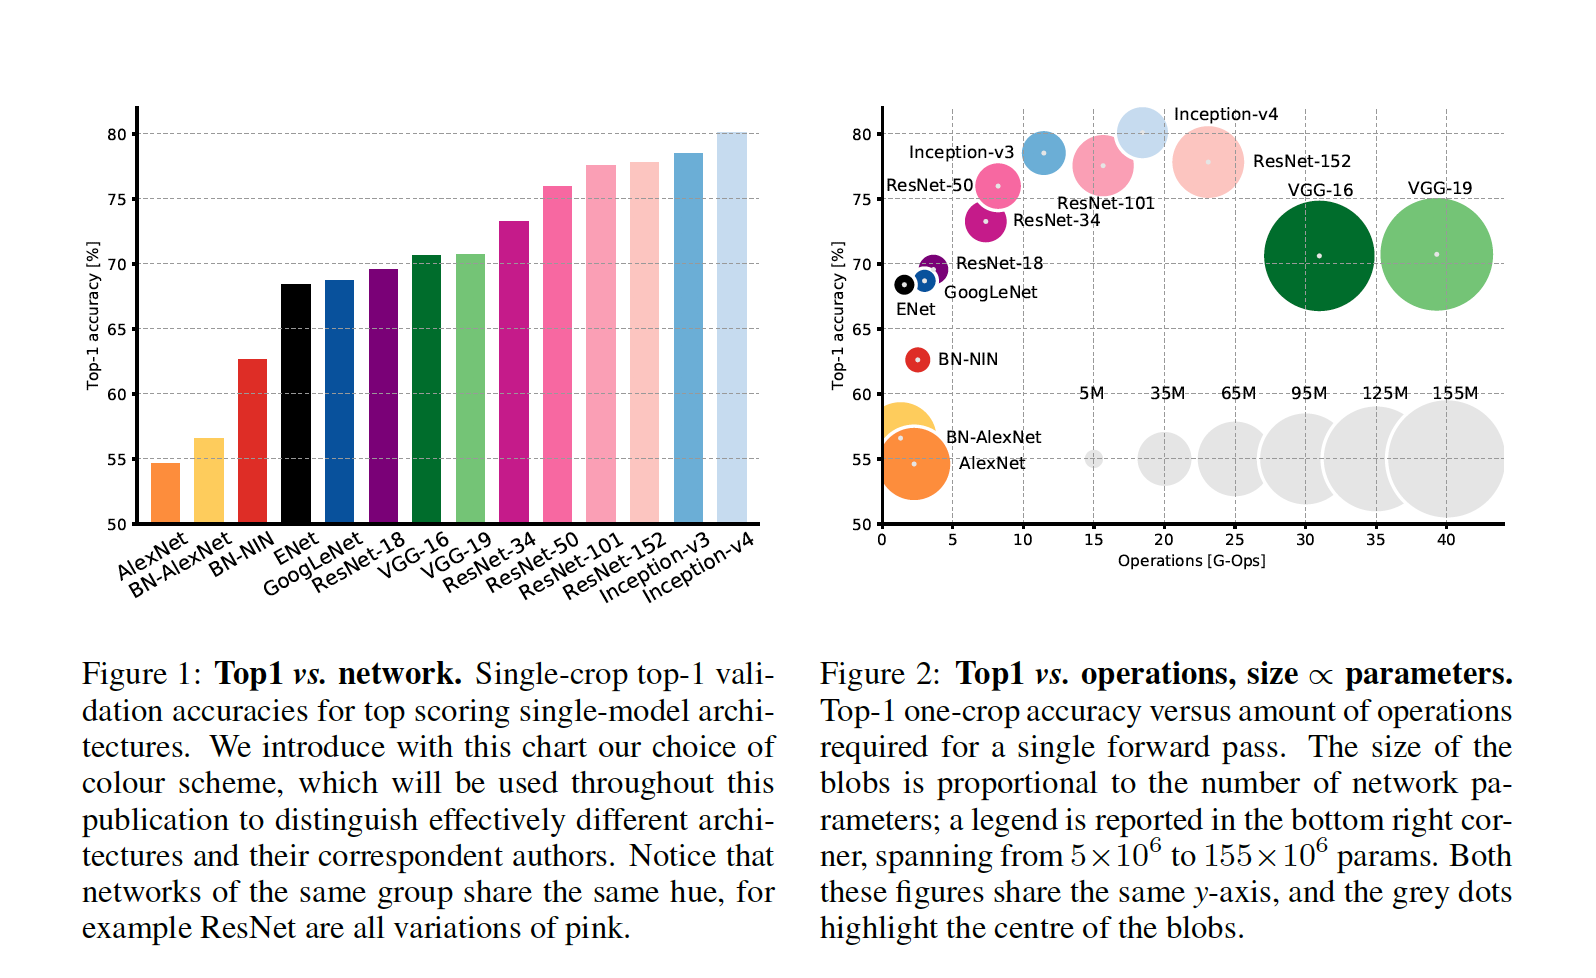
\includegraphics[scale=0.45]{figs/ic_01.png}
    \caption{}
    \label{01}
\end{figure}

\begin{figure}[!ht]
    \centering
    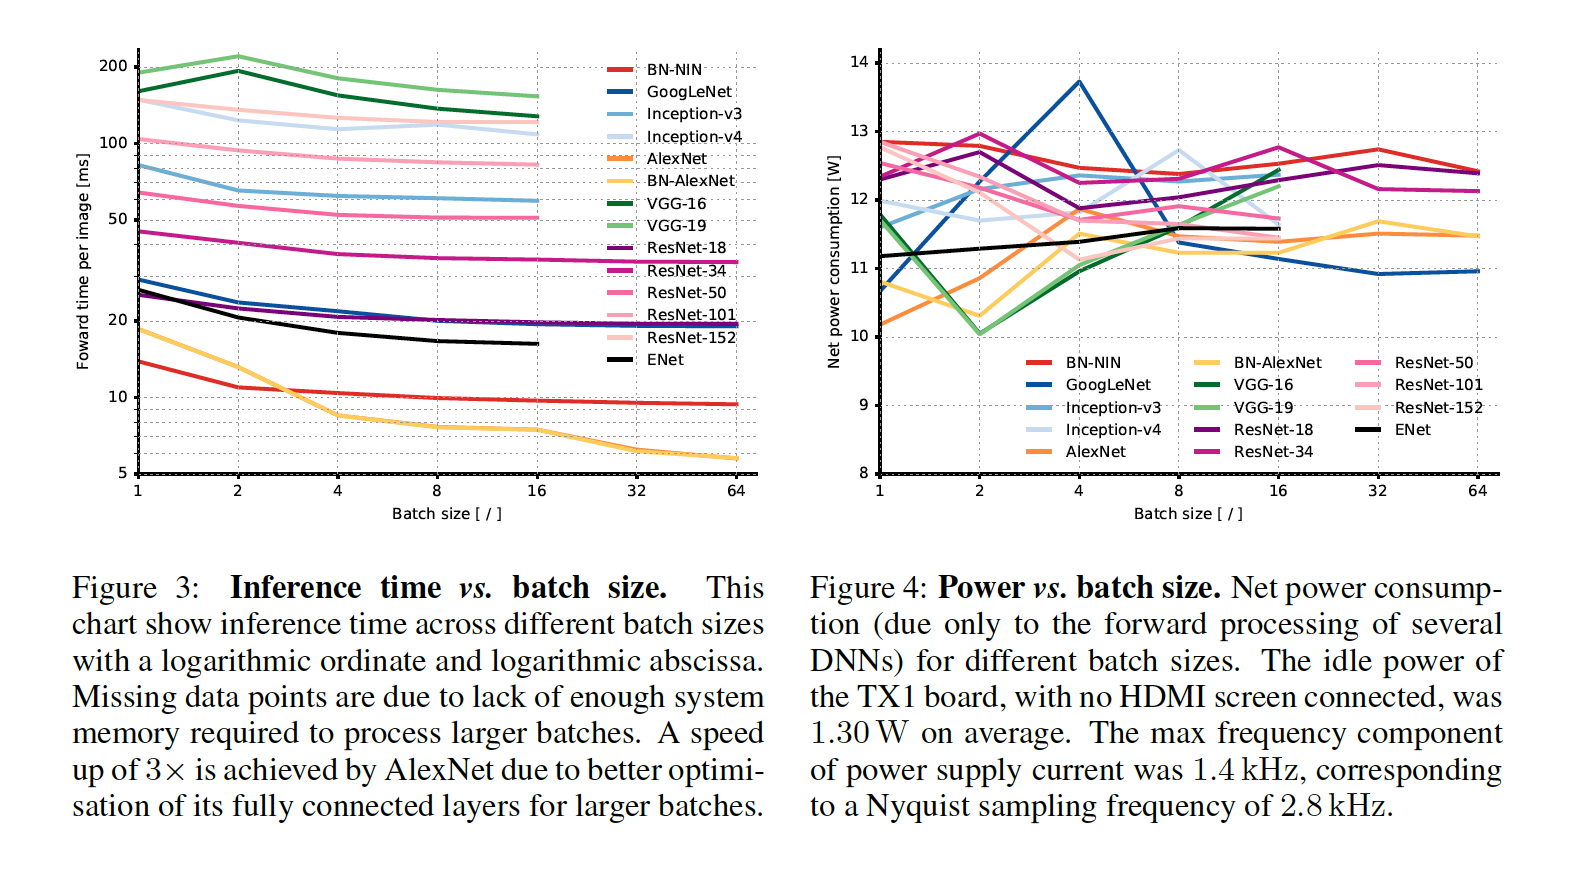
\includegraphics[scale=0.45]{figs/ic_02.png}
    \caption{}
    \label{02}
\end{figure}
\clearpage

\begin{figure}[!ht]
    \centering
    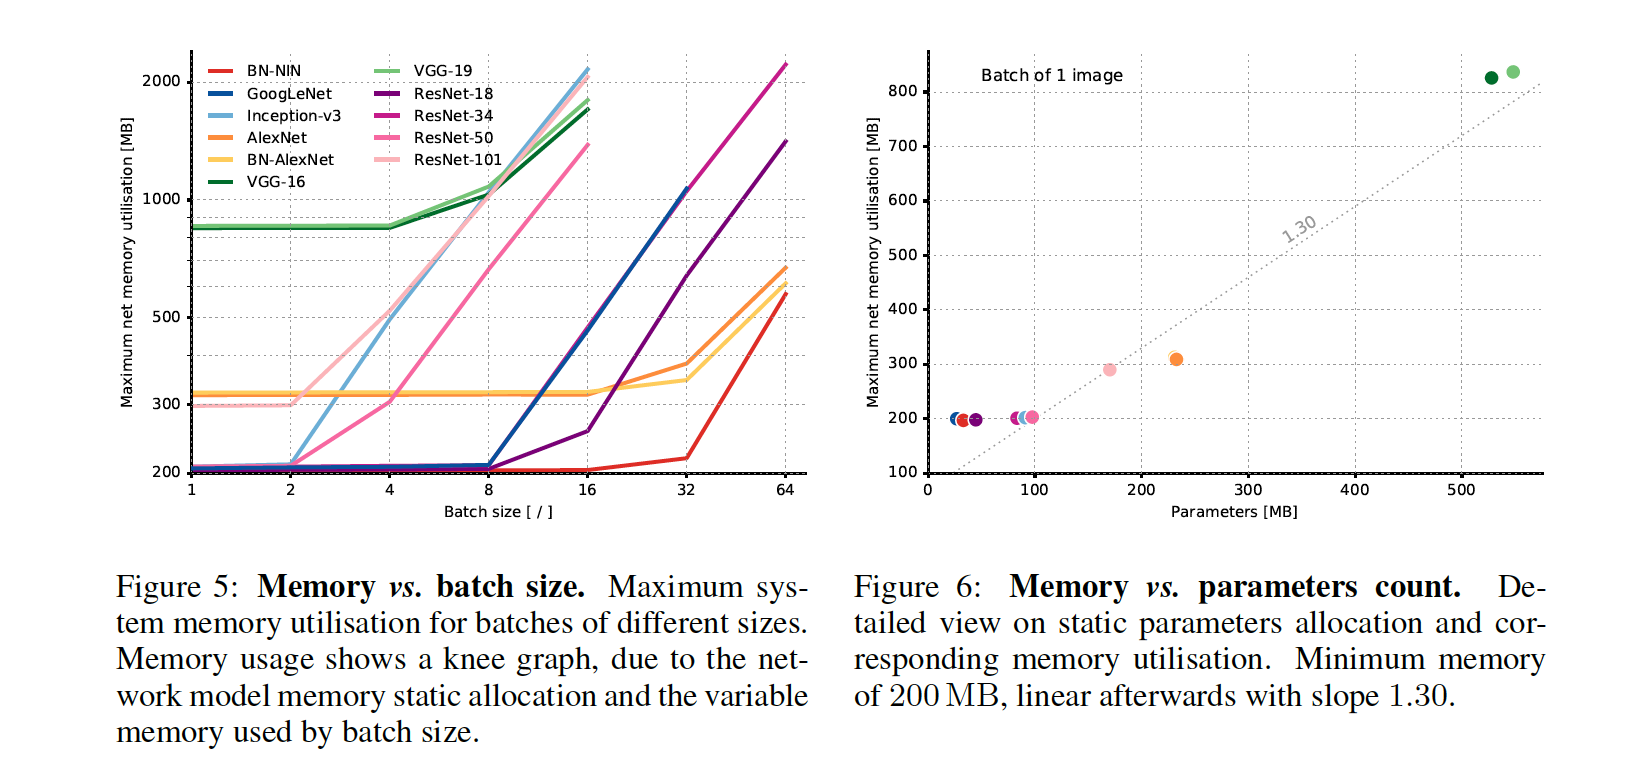
\includegraphics[scale=0.55]{figs/ic_04.png}
    \caption{}
    \label{04}
\end{figure}

\begin{figure}[!ht]
    \centering
    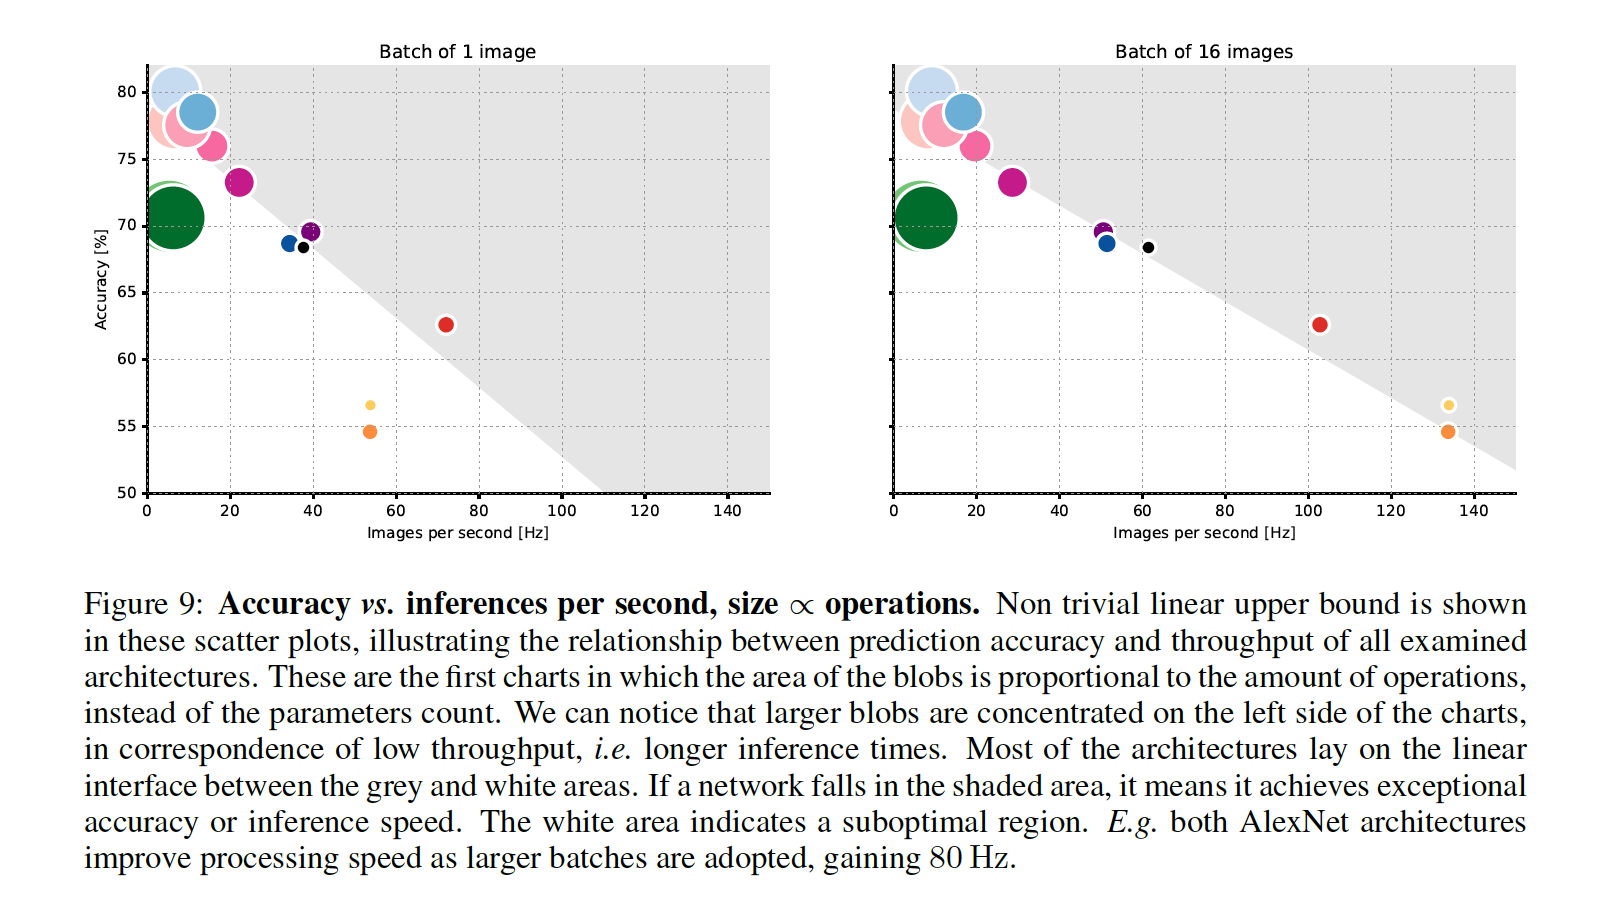
\includegraphics[scale=0.55]{figs/ic_03.png}
    \caption{}
    \label{03}
\end{figure}
\clearpage

\begin{itemize}
    \item \textbf{Accuracy:} A linear fit of the accuracy shows all architectures trade accuracy for speed (figure \ref{03}). Since power consumption is constant, we can presume that there exists a theoretical upper bound in accuracy when there is an energy constraint.
    \item \textbf{Inference time:} There is a 3 fold improvement for BN-AlexNet when batch size is increased, as shown in figure \ref{02}. 
    \item \textbf{Power Consumption:} Lower power consumption is associated with slower forward times per image. Low power consumption networks are preferred for mobile devices, and thus, people start to pay more attention to this matter as there is an increasing demand to implement neural networks on mobile devices.
    \item \textbf{Memory:} In figure \ref{04}, the initial allocation of the memory is never less than 200 MB. From a certain point, the memory required starts to grow proportionally with the number of images/batches. Memory becomes a crucial constraint when we want to employ neural networks on mobile devices. In addition, to calculate the size of the networks, we multiply the number of parameters by 4. For example, the size of GoogLeNet is 20 MB (5 million parameters time 4).
    \item \textbf{Operations:} There is a linear relationship between operations count and inference time per image.
    \item \textbf{Parameters:} Parameters utilization is closely related to information density in Deep Neural Network. It is also inefficient to not use the full learning power when training the parameters. A more compact architecture is often wanted in newer design of Deep Neural Nets. 
\end{itemize}
\section{Residual(skip) Connections}

Now we introduce the concept of \textbf{residual connections}.

In general, the more hidden layers a neural network has, the more accurate prediction it can yield. As a result, people often favor a deeper neural network as opposed to a shallower one. Nevertheless, problems may arise when the neural network attempts to learn a simple function, where adding more layers to the network often leads to lower accuracy. This is known as the \textit{degradation problem}.

\begin{figure}[ht]
    \centering
    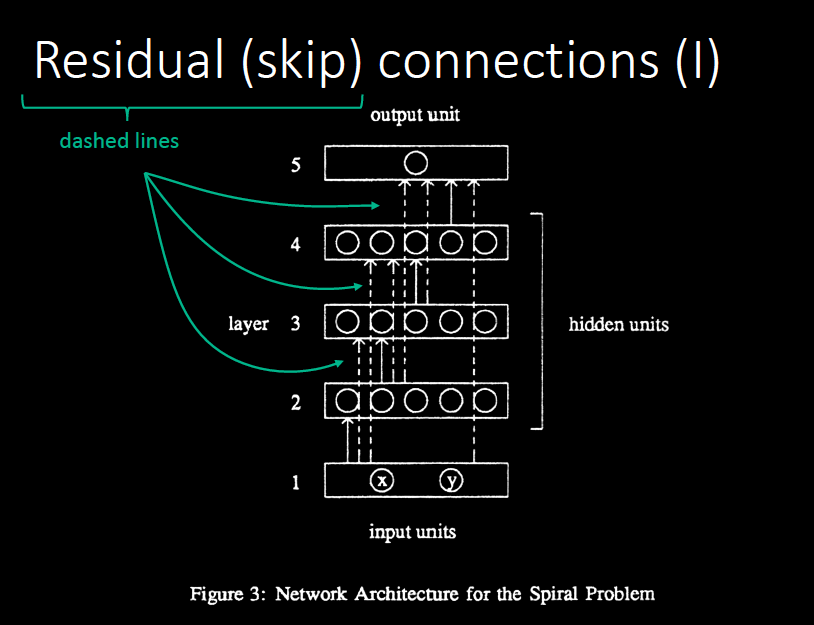
\includegraphics[scale=0.3]{figs/skip_connection.png}
    \caption{}
    \label{05}
\end{figure}

One popular solution is to skip a few hidden layers at training time, as shown in figure \ref{05}. In the residual net, the residual layer tries to learn from residual $R(x)$ rather than the true output $H(x)$. Hence, it is called the \textit{residual block}.

In other words, we provide an alternate route to some of the hidden layers -- an identity function. When some layers proved to be counterproductive, the identity function of the previous layer will take over and pass to the next layer. By doing so, we can achieve a faster computation time and generate a smoother loss surface.

\begin{figure}[!htb]
    \centering
    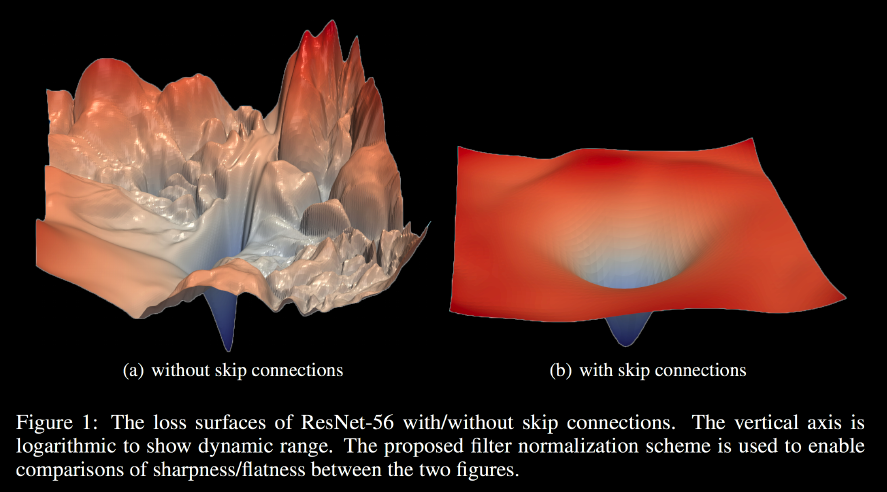
\includegraphics[scale=0.3]{figs/with_and_without_skip.png}
\end{figure}

The two graphs illustrate the loss surfaces obtained with and without skipping connections. Note that, by skipping a number of hidden layers, we end up with a much smoother loss surface compared to the one resulting from the absence of skip connections. Therefore, skip connection is an extremely useful practice in training a deep neural network.
\clearpage

\section{Summary}
% Authors: Danfeng Li, Zexi Ye, Wei-Yun Wang3/12/19.
A neural network heavily relies on computational power and data. Neural networks are often used to classify images, yet we inevitably face a trade-off between accuracy and other practical considerations such as memory. A batch size sufficiently large is required to optimize the performance of a neural network. To smooth a loss surface, we often conduct skip connections.